\documentclass[11pt]{article}
\usepackage[a4paper, margin=1in]{geometry}
\usepackage{graphicx}
\usepackage{subcaption}
\usepackage{tabularx}
\usepackage{amsmath}
\usepackage{hyperref}
\usepackage{fontawesome}

\title{Vision assignment 2}
\author{sumanasekarawkgg.19 }

\begin{document}

\begin{center}
    \textbf{EN2550 - Fundamentals of Image Processing and Machine Vision}
    {\fontsize{14.4}{18}\selectfont\textbf{\\Assignment II\\}}
    \textbf{Fitting and Alignment} \\
\end{center}

\noindent \textbf{Name}: Sumanasekara W.K.G.G. \\
\noindent \textbf{Index}: 190610E \\
\newline
\noindent \textbf{Note}: All codes relevant to this assignment can be found in \faGithub{ \url{https://github.com/GevinduGanganath/EN2550/tree/main/Assignment%202}} \\

\noindent \textbf{Question 1}

\noindent In the first part of the assignment,  a circle is estimated using the RANSAC algorithm. Objective is to write a code for RANSAC manually.
Figure \ref{RANSAC code} shows the python code written for the RANSAC algorithm. 

\begin{figure}[!h]
    \centering
    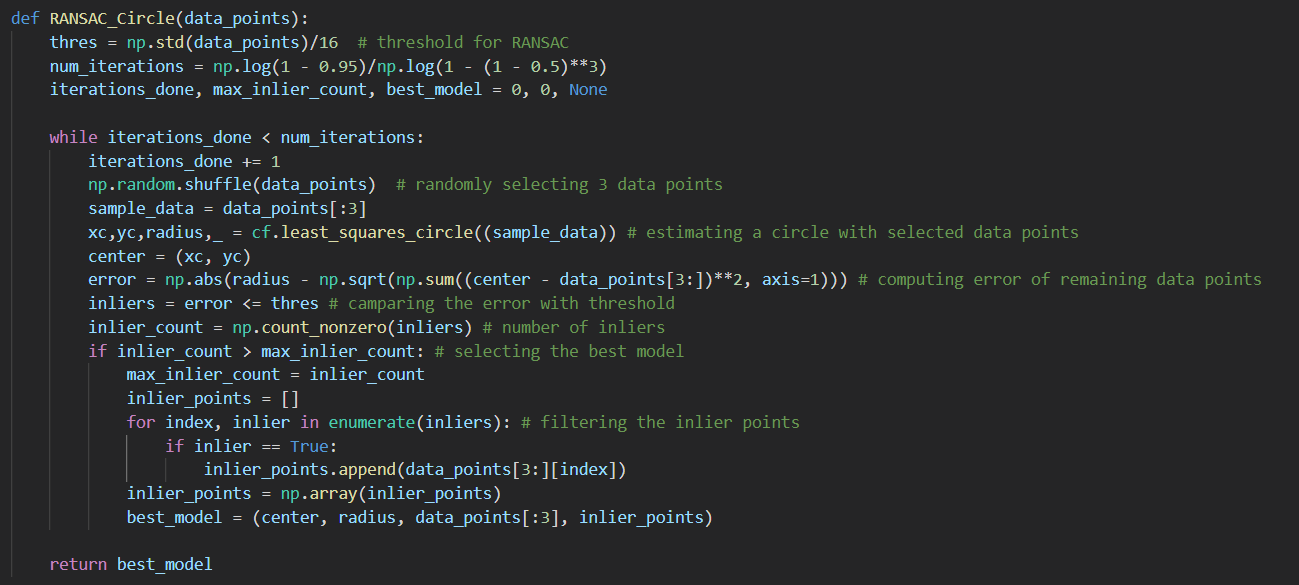
\includegraphics[width=0.8\textwidth]{Images/RANSAC code.PNG}
    \caption{Code snip of RANSAC algorithm}
    \label{RANSAC code}
\end{figure}

\noindent RANSAC parameters were set as follows:
\begin{itemize}
    \item Threshold: Standard deviation of data points divided by 16 (selected by trial and error)
    \item Number of samples (s): 3
    \item Probability (p): 0.95
    \item Outlier ration (e): 0.5
    \item Number of iterations $ = \frac{log(1-p)}{log(1-(1-e)^s)} \approx 22 $
\end{itemize}

\noindent Data points are shuffled at each iteration and the first three data points were selected to estimate the circle. \textit{least squares circle} 
function of the \textit{circle fit} python library was used to compute the center and radius. Then the distance between the center and the remaining 
data points are calculated. By comparing those values with the threshold we can count the number of inliers. The iteration which gives the highest
number of inliers was selected and using those inliers best model can be calculated. 

\noindent Figure \ref{RANSAC} shows the results. Circle obtained by RANSAC algorithm (red) is giving better results than the best samples (green). \\

\begin{figure}[!h]
    \centering
    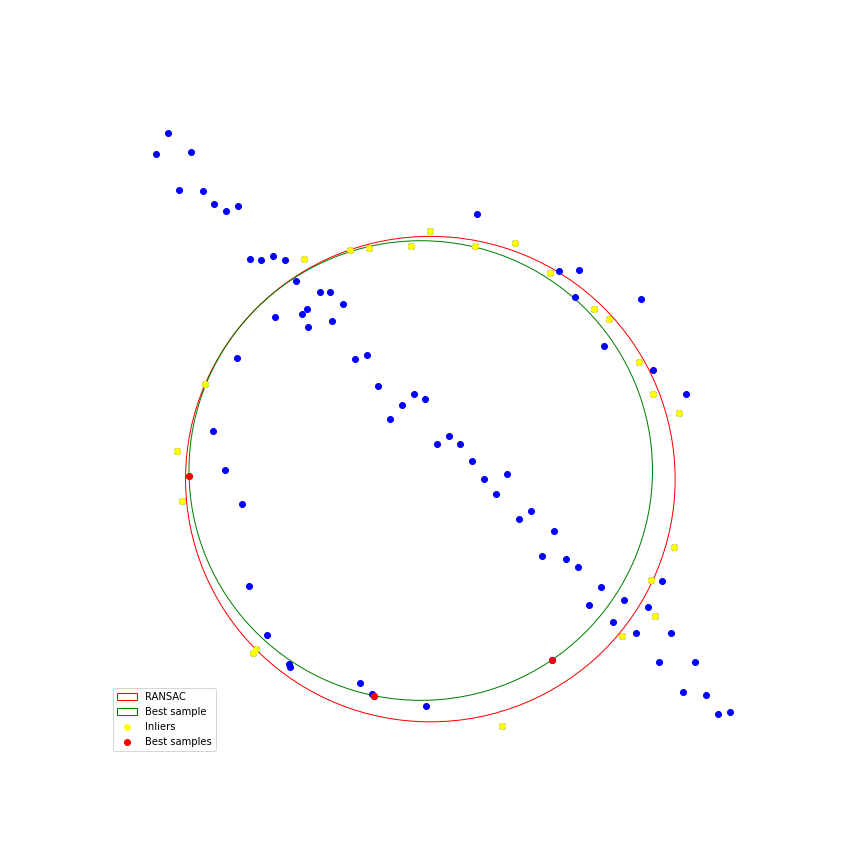
\includegraphics[width=0.6\textwidth]{Images/1.png}
    \caption{Question 1 results}
    \label{RANSAC}
\end{figure}

\newpage
\noindent \textbf{Question 2}

\noindent In this question the expectation is to superimpose a flag to an architectural image. The procedure for this is to first take four ponts
on the architectural image to compute the homography which maps the flag to architectural image. Then we can wrap the flag and blend it with architectural
image. 

\noindent Figure \ref{Q2} shows the results of the superimposing. The left column shows the point selections while the right column shows
the flag superimposed into the selected locations. \\

\begin{figure}[!h]
    \centering
    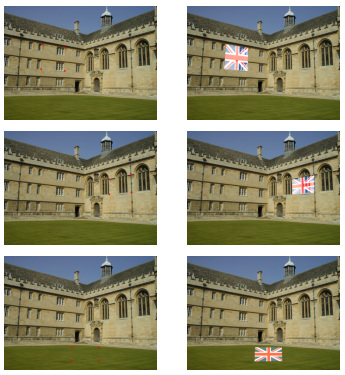
\includegraphics[width=\textwidth]{Images/2.png}
    \caption{Question 2 results}
    \label{Q2}
\end{figure}

\newpage
\noindent \textbf{Question 3}

\begin{itemize}
    \item[(a)] In the first part of question 3, it is required to compute and match SIFT features between Graffiti image 1 and 5.
    We can directly occupy openCV built-in functions for this purpose. First we have to find the keypoints and descriptors of each image. Then we
    can match these descriptors and filter them based on the distance to obtain the best results. Figure \ref{SIFT feature matching} shows the 
    results of SIFT feature matching.

    \begin{figure}[!h]
        \centering
        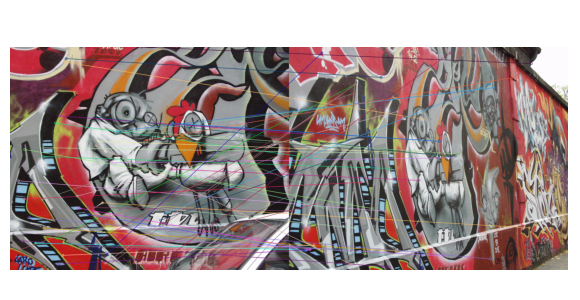
\includegraphics[width=\textwidth]{Images/31.png}
        \caption{SIFT feature matching}
        \label{SIFT feature matching}
    \end{figure}

    \item[(b)]
    \item[(c)] Graffiti image 1 was stitched into the fifth one. Initially, image 1 was wrapped using the given homography. Then we can blend it 
    with the fifth image. However, while this blending the brightness of the stitched area was increased drastically and gave an unexpected appearance.
    Therefore, the brightness of the stitching area of image 5 was reduced. Result is shown in figure \ref{Image stitching}. In the stitched image 
    we can clearly observe a part on a vehicle which has been come from image 1. 
    
    \begin{figure}[!h]
        \centering
        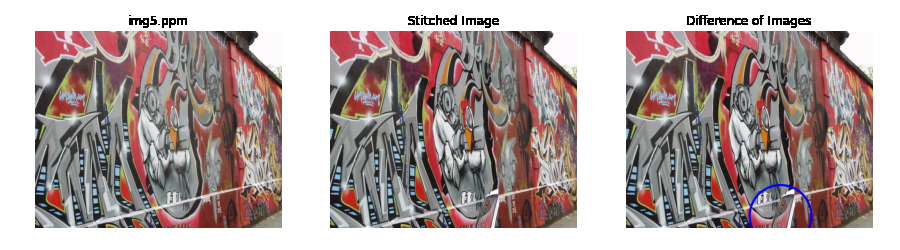
\includegraphics[width=\textwidth]{Images/33.png}
        \caption{Image stitching}
        \label{Image stitching}
    \end{figure}
      
\end{itemize}

%\newpage
%\bibliographystyle{IEEEtran}
%\bibliography{ref}

\end{document}